\documentclass{tufte-handout}
\usepackage{amsmath}
\pagestyle{empty}
\usepackage[utf8]{inputenc}
\usepackage{mathpazo}
\usepackage{microtype}

\usepackage{tikz}
\usetikzlibrary{matrix}
\usetikzlibrary{chains}
\usetikzlibrary{decorations}

\title{Word Ladders}
\author{Thore Husfeldt}

\begin{document}

\maketitle

\subsection{Description}
Find paths between given words among the five-letter words of English.

\begin{marginfigure}
  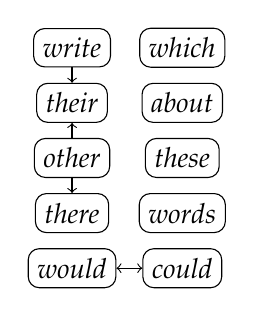
\begin{tikzpicture}[ scale=.7, 
  					   every node/.style={draw,rounded corners,font=\em}]
  \node (would) at (0,1) {would};
  \node (could) at (2,1) {could};
  \node (there) at (0,2) {there};
  \node (other) at (0,3) {other};
  \node (their) at (0,4) {their};
  \node (write) at (0,5) {write};
  \node (words) at (2,2) {words};
  \node (these) at (2,3) {these};
  \node (about) at (2,4) {about};
  \node (which) at (2,5) {which};
  \draw [<->] (would) -- (could);
  \draw [->] (other) -- (there);
  \draw [->] (other) -- (their);
  \draw [->] (write) -- (their);
  \end{tikzpicture}
  \caption{words-10.}
\end{marginfigure}

\subsection{How words connect}

We define a directed graph of words as follows.
There is one node for every 5-letter word.
There is an arc from $v$ to $w$ if each of the last four letters of $v$ appears in $w$.
For example, there is an arc from \emph{yodel} to \emph{lodes}, but not from \emph{lodes} to \emph{yodel} because the latter contains no S. 
On the other hand, there is an arc from \emph{sharp} to \emph{graph} and back. 
All four letters have to appear with repetitions, so there is an arc from \emph{where} to \emph{ether} (both Es appear) but not to \emph{retch} (E appears only once).
As an example, here’s a pretty long path in the graph: 
\bigskip

\begin{fullwidth}
\begin{quotation}\em
climb $\rightarrow$ blimp $\rightarrow$ limps $\rightarrow$ pismo $\rightarrow$ moist $\rightarrow$ stoic $\rightarrow$ ioctl $\rightarrow$ colts $\rightarrow$ lotsa $\rightarrow$ stoae $\rightarrow$ oaten $\rightarrow$ neath $\rightarrow$ hated $\rightarrow$ dated $\rightarrow$ dater $\rightarrow$ rater $\rightarrow$ tread $\rightarrow$ dared $\rightarrow$ dread $\rightarrow$ drear $\rightarrow$ rarer $\rightarrow$ reran $\rightarrow$ arena $\rightarrow$ earns $\rightarrow$ snarf $\rightarrow$ franc $\rightarrow$ narco $\rightarrow$ orcas $\rightarrow$ scare $\rightarrow$ raced $\rightarrow$ decaf $\rightarrow$ fecal $\rightarrow$ eclat $\rightarrow$ talcs $\rightarrow$ clasp $\rightarrow$ psalm $\rightarrow$ slams $\rightarrow$ small $\rightarrow$ llama $\rightarrow$ lamas $\rightarrow$ amass $\rightarrow$ smash $\rightarrow$ shame $\rightarrow$ hames
\end{quotation}
\end{fullwidth}

\subsection{Requirements}

You build a directed graph representing the adjacency structure of the words in the list called {\tt words-5757.txt}, and run BFS on it. 
The input to your algorithm is two words, like {\tt climb} and {\tt hames}.
Your algorithm returns the words on a shortest path from the first word to the second.

The data directory contains a number of test inputs with known distances, your algorithm must work correctly on those.\sidenote{There can be many shortest paths, so it makes no sense to specify the words on the path.}

If you can, make the running time of your algorithm  $O(n+m)$, where $n$ and $m$ refer to the number of nodes and arcs in the underlying directed graph. 
In particular, you’re not supposed to use quadratic time in $n$ to build the graph, even though it’s tempting.\sidenote{Of course, for dense graphs, $O(n+m)$ would be quadratic time anyway.
But the input graph is not dense.}

\subsection{Deliverables}

\begin{enumerate}
  \item The source code for your implementation
  \item A report in PDF.
  Use the report skeleton in the {\tt doc directory}.
  \end{enumerate}

\newpage
\begin{figure*}
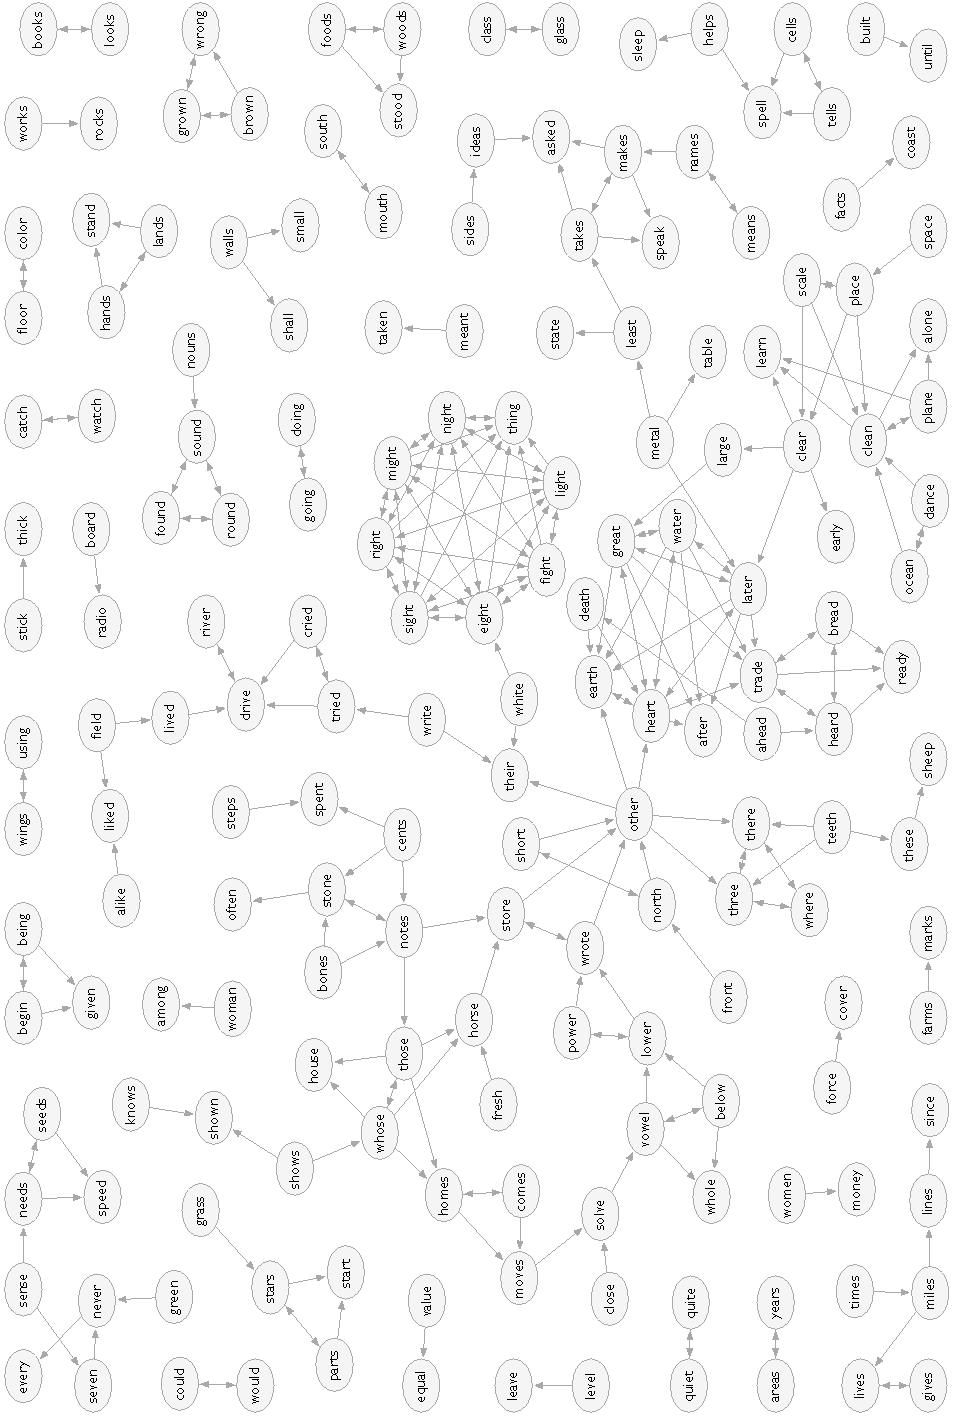
\includegraphics{words-250-layout.pdf}
\caption{words-250.}
\end{figure*}
\end{document}
